\chapter{Method}
\label{sec:method}
As explained in \Cref{sec:introduction} the aim of this work is to find a drone
design that is the result of an optimization problem, which tends to maximize the
MAV's omni-directionality, flight efficiency and controllability. To do so it is
important to first state what are the parameters that define the design of an MAV.
These parameters are defined as:

\begin{itemize}
\item $\beta$  (angles formed by the arms with the horizontal plane see \Cref{fig:drone_design})
\item $\theta$ (angles formed by the arms in the horizontal plane see \Cref{fig:drone_design})
\item $L$ (arm length)
\item $n$ (number of propeller)
\end{itemize}

\begin{figure}[h]
\centering
\begin{minipage}[t]{0.3\textwidth}
  \centering
  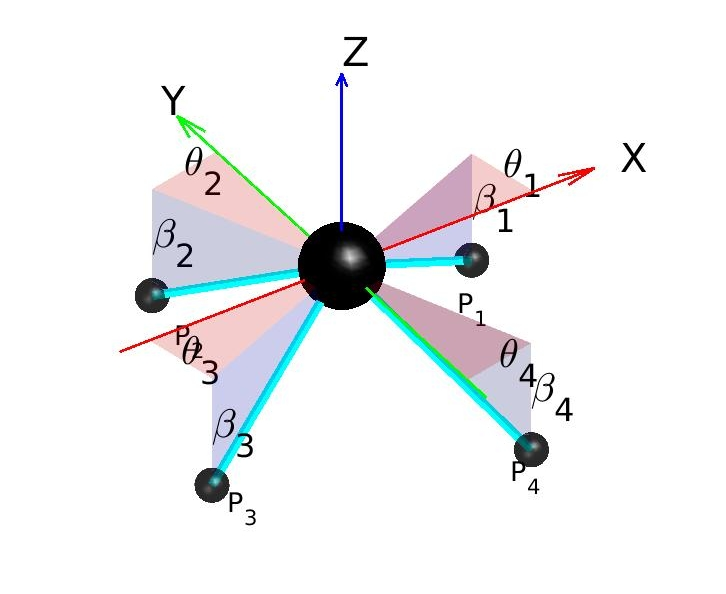
\includegraphics[width=\textwidth]{images/drone_design.jpg}
\end{minipage}
\hfill
\begin{minipage}[t]{0.3\textwidth}
  \centering
  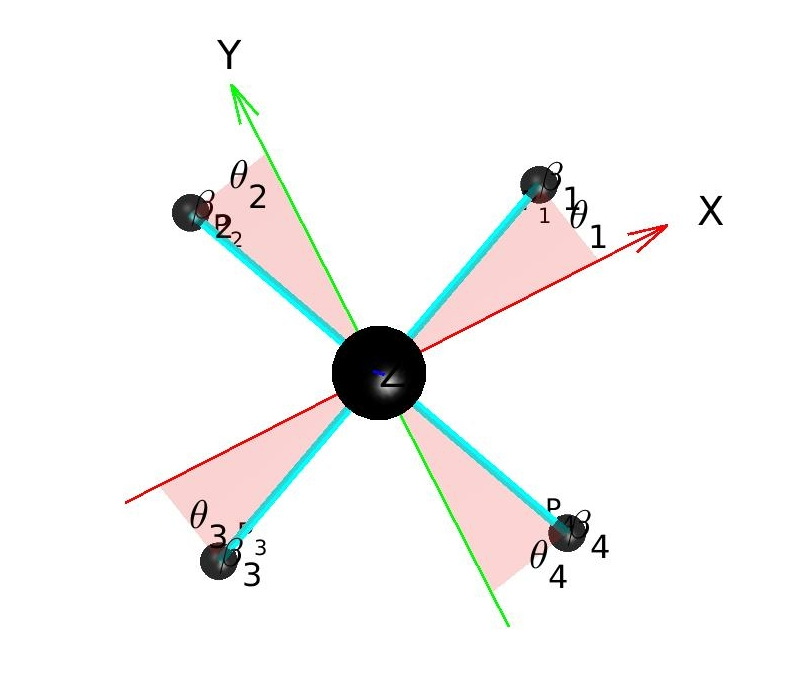
\includegraphics[width=\textwidth]{images/drone_design1.jpg}
\end{minipage}
\hfill
\begin{minipage}[t]{0.3\textwidth}
  \centering
  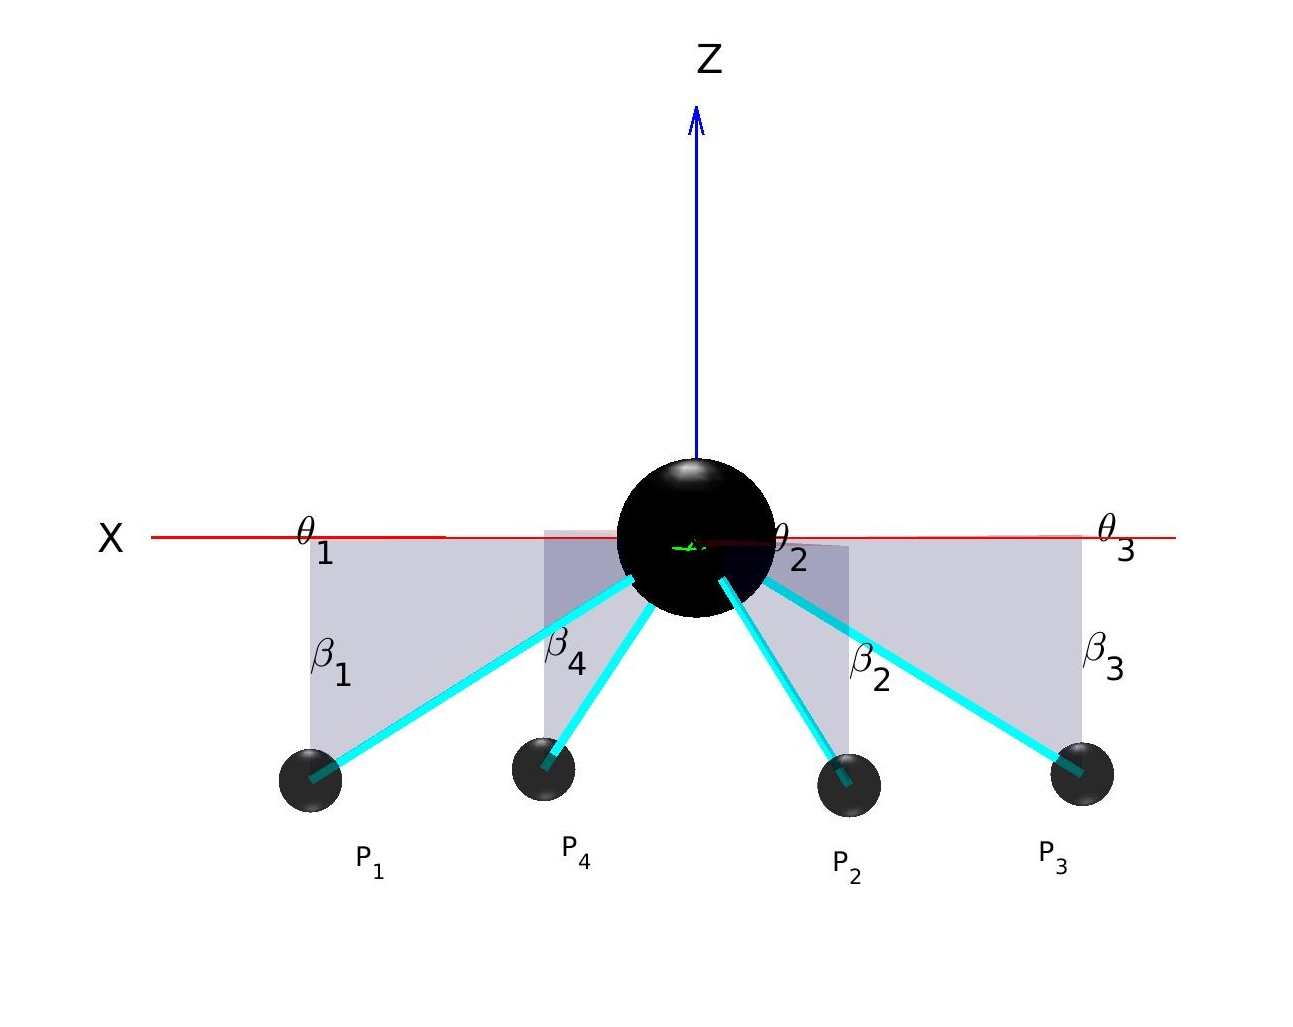
\includegraphics[width=\textwidth]{images/drone_design2.jpg}
\end{minipage}
\caption{Quadcopter to illustrate the parameters that define the morphology of an
MAV ($n = 4$, $\beta = [30, 30, 30, 30] [^{\circ}]$, $\theta = [22, 22, 22, 22]
[^{\circ}]$, and $L = 0.4 [m]$).}
\label{fig:drone_design}
\end{figure}

To solve the problem an optimization engine is developed with
MATLAB$^\textrm{\textregistered}$. This tool returns the aforementioned
parameters along with other information on the corresponding MAV design.
The interesting drone designs outputted by the tool are then simulated on
Gazebo\footnote{An open source robot simulator \citep{noauthor_gazebo_nodate}.}
and the control of the different models is achieved using a Robotic Operating
System\footnote{An open source collection of software that help developers to
create robot applications \citep{rostutorials}.} (ROS) node.\\
This chapter first covers the theory needed to obtain a generalize mathematical
model for a n-rotor MAV with an arbitrary morphology. Then, the optimization
problem is defined. Afterwards, the optimization tool is described. In the end,
the theoretical background needed to perform the simulations is covered.

\section{Modelisation of MAVs}
\label{sec:modeling_mav}
In the following part, a dynamical model for a general design of MAV is presented.
Such a modelisation is much needed to mathematiacally optimize the morphology of
a MAV. This model is inspired from the models presented in
\citep{kamel_voliro:_2018} and \citep{ryll_modeling_2012}.

\subsubsection{Assumptions}
\label{sec:assumptions}
In this model the first assumption is that the MAV is composed of n+1 rigid bodies:
one for each propeller unit $P_i$ and one for the body B. Then, it is considered that
the thrust is produced by irreversible fixed-pitch motor-propeller actuators. Finally,
only the aerodynamic forces and torques that are responsible for the MAV actuation
are considered, all the second order effects and disturbances are neglected and
also the airflow interactions between the different rotors are neglected.

\subsubsection{Initial Definitions}
\label{sec:definitions}
In order to understand correctly the dynamical model, a few definitions are much
needed. First, let us define $\mathcal{F}_{W} : \{O_{W}; X_{W},  Y_{W},  Z_{W}\}$
as the world fixed inertial frame and $\mathcal{F}_{B}: \{O_{B}, X_{B},  Y_{B},
Z_{B}\}$
as a moving frame attached to the MAV. Also, $\mathcal{F}_{P_{i}} : \{O_{P_{i}};
X_{P_{i}}, Y_{P_{i}},  Z_{P_{i}}\}, i = 1...n$ is the frame of the i-th propeller.
The propeller rotate around the axis $Z_{P_{i}}$, and thus the thrust $T_{i}$ is
produced along this axis. The tilt movement of the rotors is a simple rotation
around $X_{P_{i}}$. Now let $^{W}R_{B}$ be the orientation of the body frame
with respect to the world frame and $^{B}R_{P_{i}}$ be the orientation of the
i-th propeller with respect to the body frame. From there, it
straightforward with the help of \Cref{fig:tilt_model} that

\begin{equation}
  \label{rot_b_pi}
  ^{B}R_{P_{i}} \ = \ R_{Z}\bigg((i-1)\frac{2\pi}{n}\bigg) R_Z(\theta_i)
  R_Y(\beta_i) R_{X}(\alpha_{i}),\  i = 1...n\, .
\end{equation}

Equivalently, let

\begin{equation}
  \label{O_pi}
  ^{B}O_{P_{i}} \ = \ R_{Z}\bigg((i-1)\frac{2\pi}{n}\bigg) R_Z(\theta_i) R_Y(\beta_i)
  \begin{bmatrix}
    L \\
    0 \\
    0
  \end{bmatrix}
  ,\   i = 1...n \,
\end{equation}

be the origin of the i-th propeller frame  $\mathcal{F}_{P_{i}}$.
In \Cref{rot_b_pi} and (\ref{O_pi}), $(i-1)\frac{2\pi}{n}$ is the angle that
the i-th arm would form with axis $X_B$ if the arms of the drone are evenly
distributed in the horizontal plane, $\theta_i$ is the angle that i-th arm forms
in the horizontal plane with respect to its evenly distributed position
(see \Cref{fig:drone_design}), $\beta_i$ is the angle that the i-th arm forms with
the horizontal plane (see \Cref{fig:drone_design}), $\alpha_{i}$ is the tilting
angles of the i-th propeller about the $X_{P_{i}}$ axis, L is the arm length and
n is the number of propellers.

\begin{figure}[h]
  \centering
  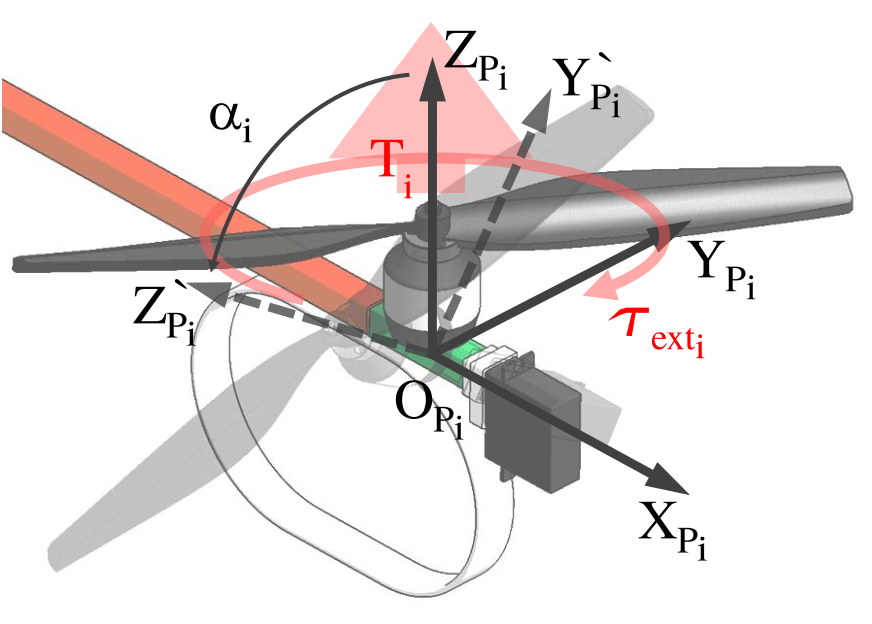
\includegraphics[width=0.4\textwidth]{images/tilt_model.png}
  \caption{Representation of the i-th tilting arm \citep{ryll_modeling_2012}.}
  \label{fig:tilt_model}
\end{figure}

\subsubsection{Equations of motion}
\label{sec:equations}
Using Newton-Euler formalism, the general equations of motion of the MAV are
\begin{equation}
  \label{acc_eq}
  \begin{cases}
    \dot{\omega}_B  \ = \ I_B^{-1} \sum_{i=1}^{n}  \big(\ ^{B}R_{P_{i}} \tau_{ext,i} + \tau_{Bi} \ \big) \, ,\\
    \ddot{p}  \ = \
    \begin{bmatrix}
      0 \\
      0 \\
      -g
    \end{bmatrix}
    \frac{1}{m} \ ^{W}R_B \sum_{i=1}^{n} T_i \, .
  \end{cases}
\end{equation}

Where

\begin{equation}
  \label{tau_b_i}
  \tau_{Bi}  \ = \ ^{B}O_{P_{i}} \times\   ^{B}R_{P_{i}} T_{P,i}\, ,
\end{equation}

\begin{equation}
  \label{tau_ext_i}
  \tau_{ext,i}  \ = \  \big[0 \ \  0 \ \  - c_i \kappa_m w_i^2 \big]^T \
\end{equation}

\centerline{ $\begin{cases} c_i = 1, & \mbox{if } i \mbox{ is odd } (cw\ rotation\ to
\ produce + thrust)\\ c_i = -1 & \mbox{if } i\mbox{ is even } (ccw\ rotation\ to
\ produce + thrust) \end{cases}$ }

and

\begin{equation}
  \label{T_i}
  T_i  \ = \ ^{B}R_{P_{i}} T_{Pi} \, ,\ \ T_{Pi}  \ = \ \big[0 \ \ 0 \ \
  \kappa_f w_i^2 \big]^T\, .
\end{equation}

In \Cref{acc_eq} $g$ is the gravity constant, in \Cref{tau_ext_i}, $\kappa_{m}$
is the propeller drag coefficient, in \Cref{T_i} $\kappa_{f}$ is the propeller
thrust coefficient and in \Cref{tau_ext_i} and (\ref{T_i}) $w_{i}$ is the i-th
propeller rotation speed.\\
The force and torque that the drone produce in body frame $\mathcal{F}_B$ are

\begin{equation}
  \label{force_eq}
    \begin{bmatrix}
      M_B \\
      F_B
    \end{bmatrix} \ = \
    \begin{bmatrix}
      \sum_{i=1}^{n}  \big(\ ^{B}R_{P_{i}} \tau_{ext,i} + \tau_{Bi} \ \big) \\
      \sum_{i=1}^{n} T_i
    \end{bmatrix}
    \, ,
\end{equation}

that can be rewritten

\begin{equation}
  \label{force_eq}
    \begin{bmatrix}
      M_B \\
      F_B
    \end{bmatrix} \ = \
    A(\alpha)W
    \, .
\end{equation}

Where $W = [w_1^2,\ w_2^2,\ ...,\ w_n^2]$ and\\\\
\centerline{\begingroup
    \fontsize{9pt}{11pt}\selectfont
$A(\alpha) \ = \
\begin{bmatrix}
  (-\kappa_f L s(\beta_1) c(\theta_1) +c_1\kappa_m s(\theta_1)) s(\alpha_1)
  + (\kappa_f L s(\theta_1) +c_1 \kappa_m c(\theta_1) s(\beta_1)) c(\alpha_1) & ...\\
  (-\kappa_f L s(\beta_1) s(\theta_1) - c_1 \kappa_m c(\theta_1)) s(\alpha_1)
  + (-\kappa_f L c(\theta_1) +c_1 \kappa_m s(\beta_1) s(\theta_1)) c(\alpha_1) & ...\\
  (-L \kappa_f c(\beta_1)) s(\alpha_1) +(c_1 \kappa_m c(\beta_1)) c(\alpha_1) & ...\\
  s(\theta_1) \kappa_f s(\alpha_1) + s(\beta_1) c(\theta_1) \kappa_f c(\alpha_1) & ...\\
  -c(\theta_1) \kappa_f s(\alpha_1) +s(\beta_1) s(\theta_1) \kappa_f c(\alpha_1) & ...\\
  c(\beta_1) \kappa_f c(\alpha_1) & ...
\end{bmatrix} \, ,$
\endgroup}\\\\
is the $6 \times n$ allocation matrix and $c(\cdot)$ and $s(\cdot)$ represent the
cosine and sine operator respectively.

\subsubsection{Static allocation}
\label{sec:allocation}
The optimization engine has to compute the maximal reachable force and torque in
a large number of direction. So to compute that in a reasonable times in
\citep{kamel_voliro:_2018} an approach to transform the non-linear allocation matrix
into a static allocation matrix, which renders the problem of inverse kinematic
linear. To do so, the system in \Cref{force_eq} is rewritten as

\begin{equation}
  \label{static_force_eq}
    \begin{bmatrix}
      M_B \\
      F_B
    \end{bmatrix} \ = \
    A_{static}F_{dec}
    \, .
\end{equation}
Where $F_{dec}$ is the decomposed force vector defined as follow
\begin{equation}
  \label{f_dec}
    F_{dec} \ = \
    \begin{pmatrix}
      F_{h,1} \\
      F_{v,1} \\
      ... \\
      F_{h,n} \\
      F_{v,n}
    \end{pmatrix} \, ,
\end{equation}

with $F_{v,1}\ = \ \kappa_f cos(\alpha_i)$ the vertical force produced by the i-th
propeller and $F_{h,1}\ = \ \kappa_f sin(\alpha_i)$ the horizontal force produced
by the i-th propeller. And the static matrix defined as\\\\
\centerline{\begingroup
    \fontsize{9pt}{11pt}\selectfont
$A_{static} \ = \
\begin{bmatrix}
      -\kappa_f L s(\beta_1) c(\theta_1) +c_1\kappa_m s(\theta_1)  &
      + \kappa_f L s(\theta_1) +c_1 \kappa_m c(\theta_1) s(\beta_1)  & ... & ...\\
      -\kappa_f L s(\beta_1) s(\theta_1) - c_1 \kappa_m c(\theta_1) &
      -\kappa_f L c(\theta_1) +c_1 \kappa_m s(\beta_1) s(\theta_1)  & ... & ...\\
      -L \kappa_f c(\beta_1) & c_1 \kappa_m c(\beta_1)  & ... & ...\\
      s(\theta_1) \kappa_f & s(\beta_1) c(\theta_1) \kappa_f & ... & ...\\
      -c(\theta_1) \kappa_f  & s(\beta_1) s(\theta_1) \kappa_f & ... & ...\\
      0 & c(\beta_1) \kappa_f  & ... & ...
\end{bmatrix}\, ,$
\endgroup}\\\\
a $6 \times 2n$ matrix that is invariant for a drone design. Using the Moore-Penrose
pseudo inverse we can easily get the inverse kinematic as follow

\begin{equation}
  \label{inverse_kin}
  F_{dec}  \ = \ A_{static}^{\dagger}
    \begin{bmatrix}
      M_{des} \\
      F_{des}
    \end{bmatrix}
    \, .
\end{equation}

Which returns the decomposed force vector for a desired force and torque. Finding
the tilting angles and propellers rotation speed required to attain this desired
force and torque is then pretty straightforward

\begin{equation}
  \label{decomposition}
  \begin{cases}
    w_i^2 = \frac{1}{\kappa_f} \sqrt{F_{v,i}^2 + F_{h,i}^2} \\
    \alpha_i = atan2(F_{h,i},F_{v,i})
  \end{cases}\, .
\end{equation}

\section{Optimization problem}
\label{sec:optimization_problem}
The following section focuses on the optimization problem that the engine has to
solve in order to obtain a MAV design that is optimal. The criteria that make
this design optimal are also discussed.

\subsubsection{Problem statement}
\label{sec:problem}
 The optimization problem is stated as follow

\begin{equation}
  \label{opt_pb}
  \begin{aligned}
    & \underset{x}{\text{arg max}}
    & & f(x) &\text{subject to} &
    \begin{cases}
      c(x) \leq 0 \\
      ceq(x) = 0 \\
      A\cdot x \leq 0 \\
      Aeq \cdot x = 0 \\
      lb \leq x \leq ub\, ,
    \end{cases}
  \end{aligned}
\end{equation}

where $f(x)$ is the cost function, $x$ the argument vector, $c(x)$
the non-linear inequality constraint vector, $ceq(x)$ the non-linear equality
constraint vector, $A$ the linear inequality constraint matrix, $Aeq$ the linear
equality constraint matrix, $lb$ the lower bound vector of the arguments ($x$)
and $ub$ the upper bound vector.\\
Once the optimization problem solved, the output is the optimal argument vector
$x^*$ that maximizes the cost function $f(x)$. In our case the argument vector
$x$ is composed of the MAV's morphology parameters ($\beta$, $\theta$, $L$, $n$)
and cost functions are the subject of next section.

\subsubsection{Cost Functions}
\label{sec:cost_functions}
As stated in \Cref{sec:introduction} the aim of the project is to obtain a multi-rotor
design that is omni-directional. Therefore, it is the heart of the problem to
define meaningful cost functions for the optimization problem, which when
solved would return parameters for an omni-directional drone. In this section
the few cost functions that capture at best the omni-directionality are described.\\
The first, and also one of the more meaningful cost function consists in maximizing
the minimal attainable force and the minimal attainable torque that the MAV can
produce in any direction. It makes sense because on of the definition of
omni-directionality  is defined as the drone capacity to accelerate instantaneously
in every directions. In order to do that the MAV has to have high minimal attainable
force and torque, hence this cost function. It turns out this cost function is also
computationally quite lighter than the other. Indeed, as when the multi-rotor apply a
force or torque in the direction parallel to one of its arm, the propeller on this arm
is perfectly unable to produce any force or torque in this direction. This is due to
the fact that no matter what the tilting angle for this propeller is, the thrust it
produces is parallel to the arm direction (see \Cref{fig:tilt_model}). Therefore,
the minimal attainable forces and torques for the drone are in the direction where
it looses a propeller, i.e. the arm directions. So instead of optimizing the force
and torque in a large number of direction, it is enough for this cost function to
optimize the force and torque in $n$ directions.\\
The second cost function consist in maximizing the minimal attainable force
and the minimal attainable torque that the MAV can produce in any direction
and minimizing the MAV’s inertia. It is the same as the first cost function, but
the last term is added in order to have an easier drone to control and thus put
a criterion on the controllability.\\
The next cost function is designed to maximize the volume of the reachable
force and torque space. The force and torque spaces are two polyhedron formed
by the drone’s attainable forces and torques in every directions (see \Cref{fig:tool_outputa}
and \Cref{fig:tool_outputb}). The idea behind this cost function is to have the
biggest task space for the drone and hence increase the MAV’s ability to navigate
in any orientation and to any
position. This cost function is computationally heavy, because in order to have
precise polyhedrons for the different spaces, the forces and torques has to be
computed in 7490 directions.\\
After that a cost function that maximize the force, the torque and the hover
efficiency in all directions. The aim of this cost function
is to maximize the agility of the MAV for good disturbance rejection. Moreover,
the term that maximizes the hover efficiency is designed to give the drone design
the ability to perform manipulation efficiently in any orientation. Solving the
optimization problem for this cost function can also be computationally heavy
depending on how many directions you choose to represent “All directions”.\\
The last cost function maximizes the force and the torque in one defined
direction d. It is mostly designed to test the optimization engine as it is
computationally light and given specific directions the optimal design is
pretty straightforward. For instance if you maximize the force in the $e_z$
direction for a 4-rotor MAV, the expected optimal solution would be a standard
quadcopter.
In the presented cost functions the multi-rotor model described in
\Cref{sec:modeling_mav} is implemented in MATLAB$^\textrm{\textregistered}$
to compute the different forces and torques in the different directions.

\subsubsection{Solver}
\label{sec:solver}
In order to solve the previously described optimization problems, the tool uses
MATLAB$^\textrm{\textregistered}$ function fmincon, with different algorithm.
The one showing the quickest convergence and the best results being the sequential quadratic programming (sqp).

\section{Optimization tool}
\label{sec:optimization_tool}

\subsubsection{User Guide}
\label{sec:user_guide}

\begin{figure}[!h]
  \centering
  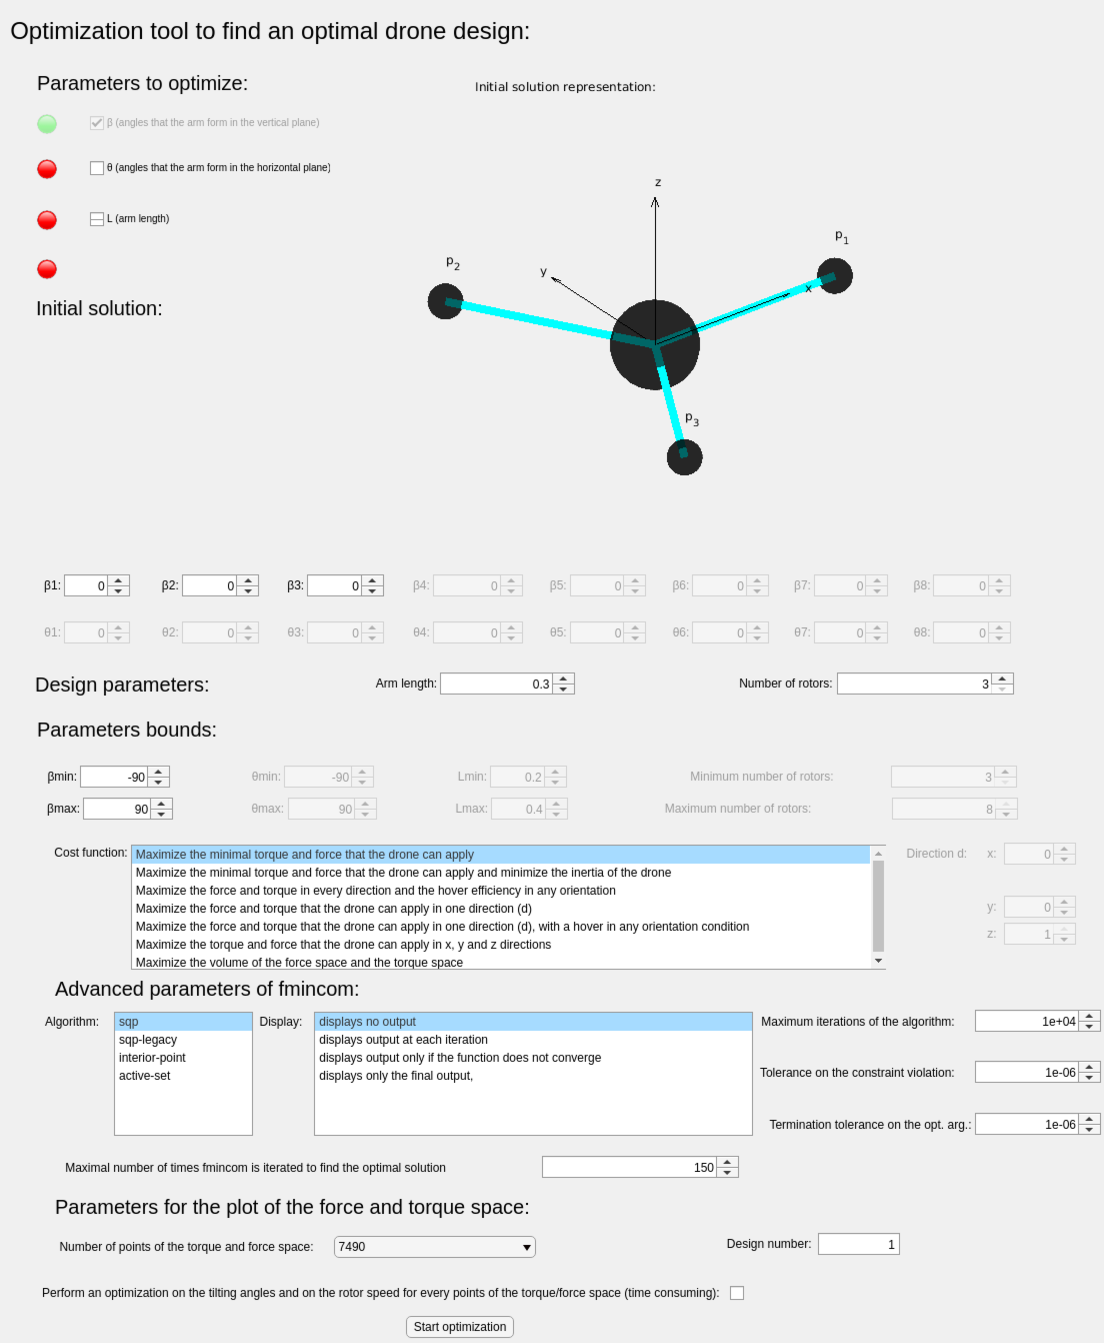
\includegraphics[width=1.0\textwidth]{images/gui.png}
  \caption{MAV morphology optimization tool GUI.}
  \label{fig:gui}
\end{figure}

\subsubsection{Outcome}
\label{sec:outcome}

\begin{figure}[!h]
  \begin{subfigure}[b]{0.48\textwidth}
    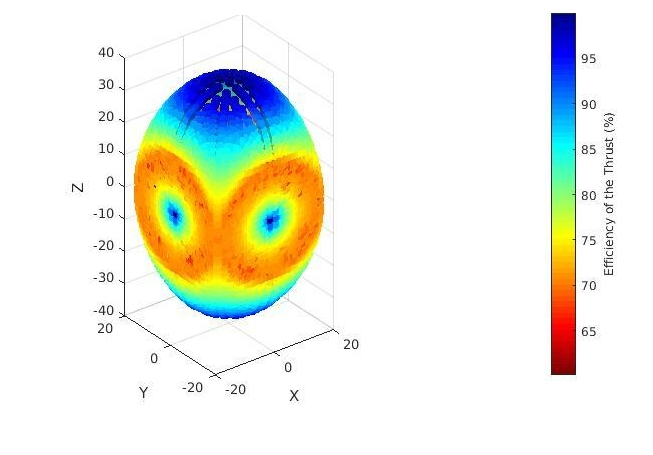
\includegraphics[width=\linewidth]{images/n=4_force.jpg}
    \caption{Force space.} \label{fig:tool_outputa}
  \end{subfigure}
  \hspace*{\fill} % separation between the subfigures
  \begin{subfigure}[b]{0.48\textwidth}
    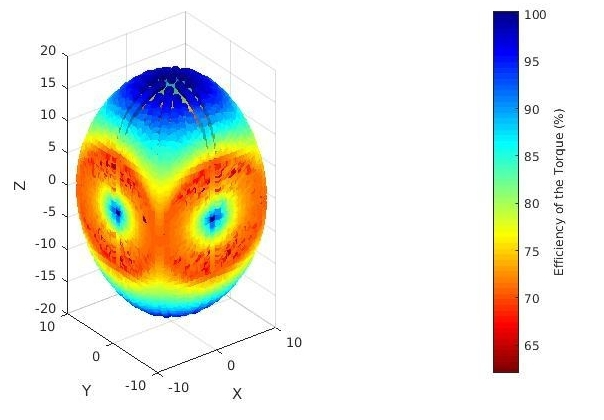
\includegraphics[width=\linewidth]{images/n=4_torque.jpg}
    \caption{Torque space.} \label{fig:tool_outputb}
  \end{subfigure}
  \hspace*{\fill} % separation between the subfigures
  \begin{subfigure}[b]{0.48\textwidth}
    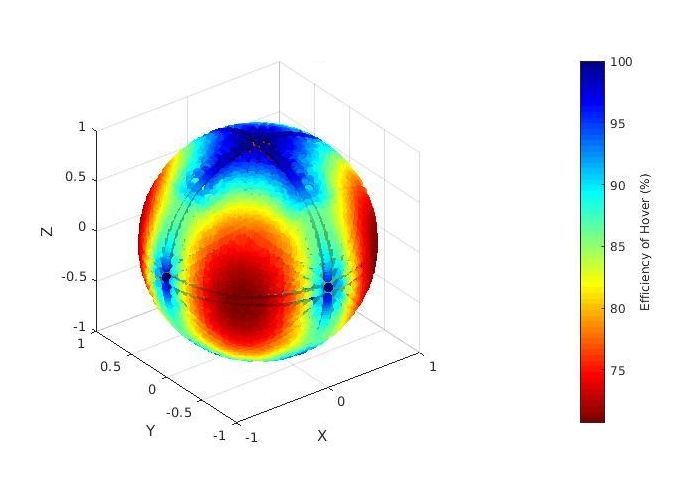
\includegraphics[width=\linewidth]{images/n=4_hover.jpg}
    \caption{Hover efficiency.} \label{fig:tool_outputc}
  \end{subfigure}
  \hspace*{\fill} % separation between the subfigures
  \begin{subfigure}[b]{0.48\textwidth}
    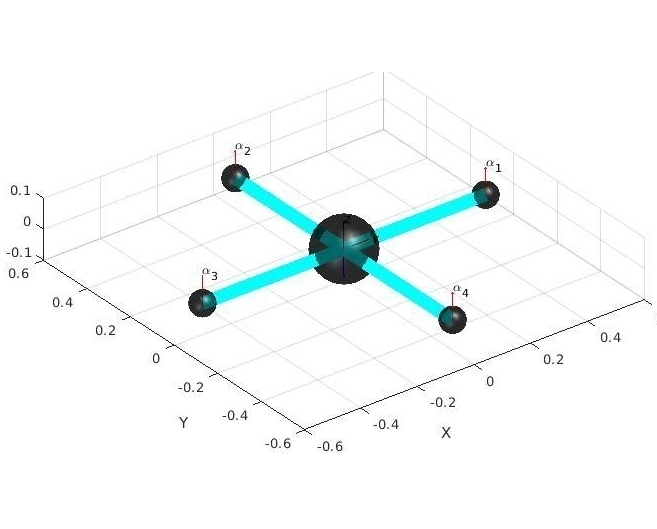
\includegraphics[width=\linewidth]{images/n=4_model.jpg}
    \caption{MAV representation.} \label{fig:tool_outputd}
  \end{subfigure}
  \caption{Example of what is outputted by the optimization engine.}
  \label{fig:tool_output}
\end{figure}

\subsubsection{Limitations}
\label{sec:limitations}

\section{Simulation Approach}
\label{sec:control_approach}
